\input{head.inc}

% Präambelbefehle für die Präsentation
\title[TET: Elektrostatik-VII: Separationsverfahren]{Elektrostatik-VII: Separationsverfahren}

\begin{document}
% 
% Frontmatter 
% 
%%%%%%%%%%%%%%%%%%%%%%%%%%%%%%%%%%%%%%%%%%%%%%%%%%%%%%%%%%%%%%%%%%%%%%%%%%%%%%%%%%%%%%%%%%%%%%%%%%%%%%%%%%%%%%%%%%%%%%%%%%%%% 

%% inserts the title page and the table of contents
\maketitle

% 
% Content 
% 
%%%%%%%%%%%%%%%%%%%%%%%%%%%%%%%%%%%%%%%%%%%%%%%%%%%%%%%%%%%%%%%%%%%%%%%%%%%%%%%%%%%%%%%%%%%%%%%%%%%%%%%%%%%%%%%%%%%%%%%%%%%%% 
\section{Elektrostatik-VII: Separationsverfahren}

\begin{frame}

  \frametitle{Problemstellung}
  \begin{itemize}[<+->]
  \item Wir untersuchen weiterhin Lösungsmethoden der \alert{Poisson-Gleichung}
    $$
    \laplace \phi = -\frac{1}{\varepsilon_0} \rho(\Ortsr[v]) \text{ in } V
    $$
    mit \alert{Dirichlet-} und/oder \alert{Neumann-Randbedingungen} auf der Oberfläche von $V$:
    $$
    \forall \Ortsr[v]_{b} \in O(V) : \phi(\Ortsr[v]_b) \veebar \left. \frac{\partial \phi}{\partial n}\right|_{\Ortsr[v]=\Ortsr[v]_b} \text{ vorgegeben}
    $$
  \item In Fällen, in denen die Problemgeometrie gut zu den Symmetrien des Koordinatensystems passt, kann sich ein \alert{Separationsansatz} bzw. \alert{Produktansatz} lohnen.
  \item Ziel ist es hierbei, die partielle Differentialgleichung in ein System gewöhnlicher Differentialgleichungen zu überführen.
  \item Randbedingungen werden dann durch geeignete Anpassung der Konstanten berücksichtigt.
    \item Ansatz für Koordinaten $(x_1,x_2,x_3)$: $\boxed{\phi(\Ortsr[v])= f(x_1) \cdot g(x_2) \cdot h(x_3) }$
    \end{itemize}
  
  \end{frame}

  \begin{frame}
    \frametitle{Laplacegleichung in 2D mit Randbedingungen}
      \vspace*{-3mm}
      
    \begin{itemize}[<+->]
    \item Wir betrachten folgendes 2D Problem:
    \begin{itemize}[<+->]
     \item Lösungsvolumen: $ V = [0,x_0] \times [0,y_0]$ (Rechteck in der $x$-$y$-Ebene)
    \item Randwerte: $\phi(x,y) = 0$ für $x=0$, $x=x_0$ und $y=0$ sowie $\phi(x,y_0) = \phi_0(x)$
    \item keine Ladungen in $V$, also $\boxed{\laplace\phi = 0 \text{ in } V}$
    \end{itemize}
  \item Mit dem Laplaceoperator $\laplace = \frac{\partial^2}{\partial x^2} + \frac{\partial^2}{\partial y^2}$ und dem \alert{Ansatz} $\phi (x,y) = f(x)g(y)$
    folgt
    \begin{align*}
      \laplace\phi(x,y)   = \laplace\left[f(x)g(y)\right] = g(y)\frac{\upd^2 f(x)}{\upd x^2} + f(x)\frac{\upd^2 g(y)}{\upd y^2} &= 0\\
      \frac{1}{f(x)}\frac{\upd^2 f(x)}{\upd x^2} + \frac{1}{g(y)}\frac{\upd^2 g(y)}{\upd y^2} &= 0\quad (\text{für } \phi\neq 0)
    \end{align*}
  \item Offensichtlich müssen die beiden Summanden sich gegenseitig aufheben:
    $$
    \boxed{- \frac{1}{f(x)}\frac{\upd^2 f(x)}{\upd x^2}  = k^2 =  \frac{1}{g(y)}\frac{\upd^2 g(y)}{\upd y^2}} \in \mathbb{R}
    $$
    \item Ein positiver Wert (oder Null) für $\frac{1}{f(x)}\frac{\upd^2 f(x)}{\upd x^2}$ führt auf den gegebenen Randbedingungen zu keiner Lösung. 
      \end{itemize}
\end{frame}

\begin{frame}
  \begin{itemize}[<+->]
  \item Allgemeine Lösung:
    \begin{align*}
      f''(x) & = - k^2 f(x) & f(x) &= \alpha \sin(kx) + \beta \cos(kx) \\
      g''(y) & = k^2 g(y) & g(y) &= \gamma\sinh(ky) + \delta\cosh(ky)
    \end{align*}
  \item Randbedingungen \enquote{links} ($x=0$), \enquote{unten} ($y=0$) und \enquote{rechts} ($x=x_0$):
    \begin{align*}
      \phi(x=0,y) &= 0 & \Aboxed{\beta &=0} \\
      \phi(x,y=0) &=0 & \Aboxed{\delta &= 0} \\
      \phi(x=x_0, y) &= 0 & \alpha\sin(kx_0) &= 0 \Rightarrow \Aboxed{k=k_n=\frac{n\pi}{x_0}}\;n\in\mathbb{N} 
    \end{align*}
  \item Die vollständige Lösung - die aber noch nicht die Randbedingung \enquote{oben} erfüllt, ist daher:
    $$
    \phi(x,y) = \sum_{n\in\mathbb{N}} c_n \sin\left( \frac{n\pi}{x_0} x \right) \sinh\left( \frac{n\pi}{x_0} y \right)
    $$
  \end{itemize}
\end{frame}

\begin{frame}
  \begin{itemize}[<+->]
  \item Die vollständige Lösung und Randbedingung \enquote{oben}:
    \begin{align*}
      \phi(x,y) &= \sum_{n\in\mathbb{N}} c_n \sin\left( \frac{n\pi}{x_0} x \right) \sinh\left( \frac{n\pi}{x_0} y \right)\\
      \phi(x,y=y_0) = \phi_0(x) &= \sum_{n\in\mathbb{N}} c_n \sin\left( \frac{n\pi}{x_0} x \right) \sinh\left( \frac{n\pi}{x_0} y_0 \right)
    \end{align*}
  \item Auflösen nach $c_n$ $\to$ Summe auf einen Term reduzieren
  \item Dazu \alert{Orthogonalität} und \alert{Vollständigkeitsrelation} nutzen $\to$ Multiplikation mit \textcolor{red}{$\sin\left( \frac{m\pi}{x_0} x \right)$} und \textcolor{green}{Integration über $[0,x_0]$}:
    \begin{align*}
      \phi_0(x) \textcolor{red}{\sin\left( \frac{m\pi}{x_0} x \right)} &= \sum_{n\in\mathbb{N}} c_n \sin\left( \frac{n\pi}{x_0} x \right) \textcolor{red}{\sin\left( \frac{m\pi}{x_0} x \right)} \sinh\left( \frac{n\pi}{x_0} y_0 \right) \\
      \textcolor{green}{\int_0^{x_0}} \phi_0(x) \textcolor{red}{\sin\left( \frac{m\pi}{x_0} x \right)} \textcolor{green}{\upd x} &=
                                                                                                                                   \sum_{n\in\mathbb{N}} c_n \underbrace{\textcolor{green}{\int_0^{x_0}} \sin\left( \frac{n\pi}{x_0} x \right) \textcolor{red}{\sin\left( \frac{m\pi}{x_0} x \right)} \textcolor{green}{\upd x}}_{\frac{x_0}{2}\delta_{mn}} \sinh\left( \frac{n\pi}{x_0} y_0 \right) \\
      \Aboxed{c_n &= \frac{2}{x_0 \sinh\left( \frac{n\pi}{x_0} y_0 \right)}  \int_0^{x_0} \phi_0(x) \sin\left( \frac{n\pi}{x_0} x \right) \upd x}
      \end{align*}
  \end{itemize}

\end{frame}

\begin{frame}
  \frametitle{Poissongleichung mit Randbedingungen $\to$ Symmetrie, formale Lösung (Green) und Separation}

  \begin{itemize}[<+->]
  \item Lösungsvolumen: $V = [-\infty,\infty] \times [0,d]\times [-\infty,\infty]$
  \item Randwerte: $\phi(x,y=0,z)=\phi(x,y=d,z) = 0$
  \item Quelle: konstante Ladungsdichte entlang $z$: $\rho_V (\Ortsr[v])
    = \rho_L \delta(x-x_0)\delta(y-y_0);\; x_0 \text{ beliebig};\; y_0
    \in (0,d)$
  \item Symmetrie: \alert{Translationsinvarianz} in $z$-Richtung: Lösung unabhängig von $z$ $\to$ \alert{2D}
    $$
    \phi(x,y,z) = \phi(x,y); \; V\to A= [-\infty,\infty] \times [0,d]; \; \rho_V \to \rho_F(x,y) = q \delta(x-x_0)\delta(y-y_0)  
    $$
  \item Möglichkeit: Formale Lösung $\to$ Greensche-Funktion z.B: durch (unendliche) Spiegelung $\to$ fertig.
  \item Alternative: Aufteilen des Lösungsgebietes in den Bereich $A_-$ \enquote{links} von $x=x_0$ und den Bereich $A_+$ \enquote{rechts} von $x=x_0$:
    \begin{align*}
      A_- &= \{\Ortsr[v] = (x,y)\; |\; x<x_0 \land 0\le y\le d \} \\
      A_+ &= \{\Ortsr[v] = (x,y)\; |\; x>x_0 \land 0\le y\le d \} 
      \end{align*}
  \end{itemize}
\end{frame}

\begin{frame}
  \begin{itemize}[<+->]
  \item Durch die Aufteilung in $A_-$ und $A_+$ muss dort \enquote{nur} noch die Laplace-Gleichung gelöst werden
    $$
    \laplace \phi_-  (x,y) = 0 \text{ für } (x,y) \in A_- ;\quad \laplace \phi_+ (x,y) = 0 \text{ für } (x,y) \in A_+ 
    $$
  \item mit den Randbedingungen
    \begin{itemize}[<+->]
    \item $\phi_\pm (x, y=0) = \phi_\pm(x,y=d) = 0 $ (Dirichlet)
    \item $\left. -\varepsilon_0\left( \frac{\partial \phi_+}{\partial x} -\frac{\partial \phi_-}{\partial x} \right)\right|_{x=x_0} = q\delta(y-y_0)=\sigma(y)$ (Neumann)
      \item $\phi_-(x\to-\infty) = 0 = \phi_+(x\to+\infty) $ (RB im Unendlichen) 
      \end{itemize}
    \item Produktansatz in der $x$-$y$-Ebene: $\phi_\pm(x,y) = f(x)\cdot g(y)$
    \item Umformen der Laplace-Gleichung: $\frac{1}{f(x)}\frac{\upd^2 f(x)}{\upd x^2}  = k^2 =  -\frac{1}{g(y)}\frac{\upd^2 g(y)}{\upd y^2}$
    \item Lösungen:
      \begin{align*}
        f(x) &= \alpha e^{kx} + \beta e^{-kx} \\
        g(y) &= \gamma\sin(ky) + \delta\cos(ky); \quad k>0 \text{ o.B.d.A.}
      \end{align*}
      \item $\phi_\pm(x,y=0) = 0 \Rightarrow \boxed{\delta=0}$, $\phi_\pm(x,y=d) = 0 \Rightarrow \boxed{k=k_n = \frac{n\pi}{d}} \text{ für } n\in\mathbb{N}$
  \end{itemize}
\end{frame}
\begin{frame}
\begin{itemize}[<+->]
\item Lösung soweit: $\phi_\pm(x,y) = \sum_{n=1}^\infty C_n^\pm \left[\alpha e^{\frac{n\pi}{d} x} + \beta e^{-\frac{n\pi}{d} x}\right]\gamma \sin\left(\frac{n\pi}{d} y\right) $
\item Mit den Randbedingungen $\phi_-(x\to -\infty, y) = 0 = \phi_+(x\to+\infty, y) $:
  $$
  \phi_\pm(x,y) = \sum_{n=1}^\infty C_n^\pm e^{\mp\frac{n\pi}{d} x} \sin\left(\frac{n\pi}{d} y\right)
  $$
\item Die Lösung muss bei $x=x_0$ stetig sein:
  $$
  \sum_{n=1}^\infty C_n^+ e^{-\frac{n\pi}{d} x_0} \sin\left(\frac{n\pi}{d} y\right) = \sum_{n=1}^\infty C_n^- e^{+\frac{n\pi}{d} x_0} \sin\left(\frac{n\pi}{d} y\right)  
  $$
  \item Dies erfordert:
  $$
C_n^+ e^{-\frac{n\pi}{d} x_0} = C_n^- e^{+\frac{n\pi}{d} x_0} = A_n; \; \forall n\in\mathbb{N}  
$$
\item Damit:
  $$
  \phi_\pm(x,y) = \sum_{n=1}^\infty A_n e^{-\frac{n\pi}{d} |x-x_0|} \sin\left(\frac{n\pi}{d} y\right)
  $$
\item Mit $\left. -\varepsilon_0\left( \frac{\partial \phi_+}{\partial x} -\frac{\partial \phi_-}{\partial x} \right)\right|_{x=x_0} = q\delta(y-y_0)=\sigma(y)$ und der Orthonormalitätsbeziehung:
  \begin{align*}
    A_n &= \frac{q}{\varepsilon_0 \pi} \frac{\sin\left(\frac{n\pi}{d}y_0\right)}{n} \\
    \Aboxed{\phi(x,y) &= \frac{q}{\varepsilon_0 \pi}  \sum_{n=1}^\infty \frac{1}{n} \sin\left(\frac{n\pi}{d}y_0\right)  \sin\left(\frac{n\pi}{d}y\right)  e^{-\frac{n\pi}{d} |x-x_0|} } \; \vec{E} = -\gradient\phi
    \end{align*}
  \end{itemize}
  \end{frame}

  \begin{frame}

    \only<1|handout:0>{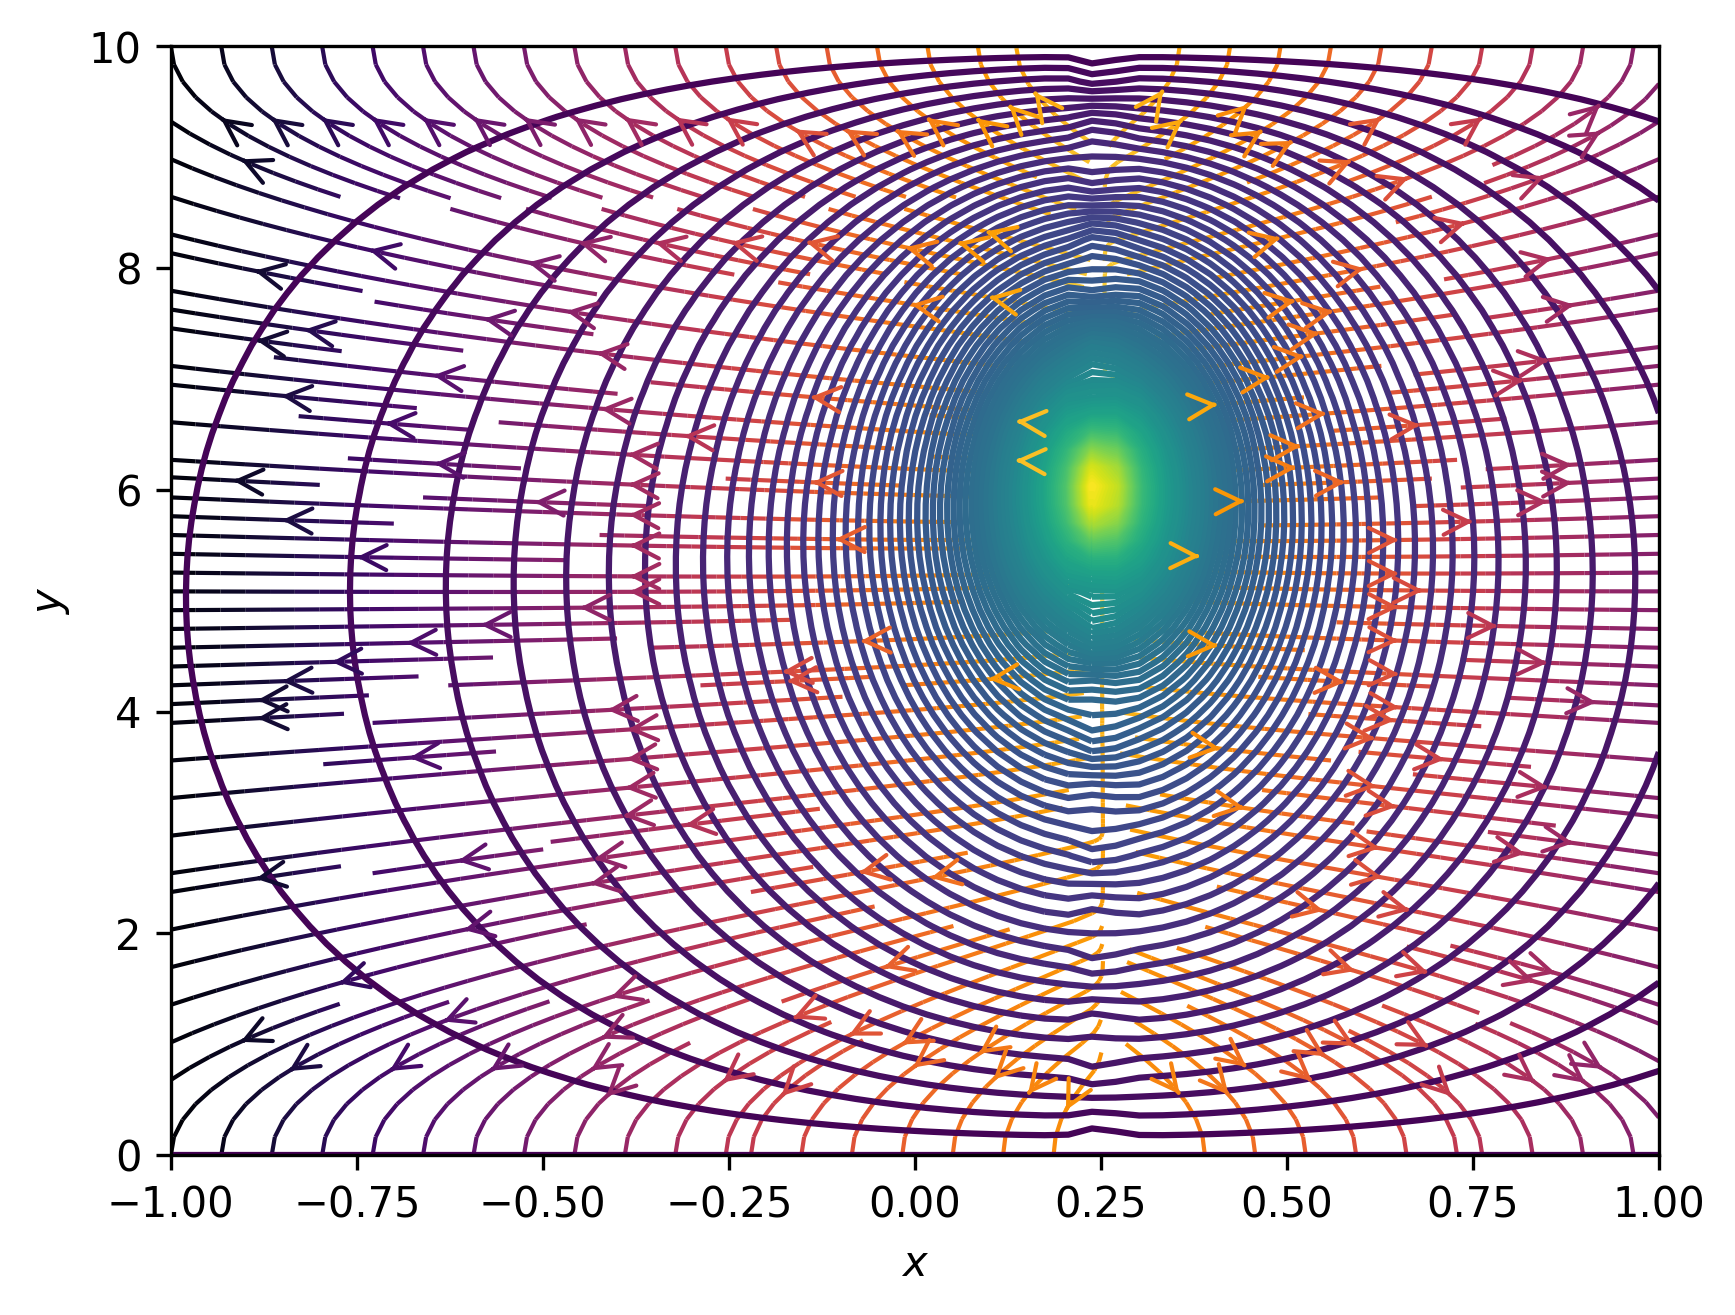
\includegraphics[width=\linewidth]{programs/estatic-wire-plates/plate-wire-20.png}}\only<2>{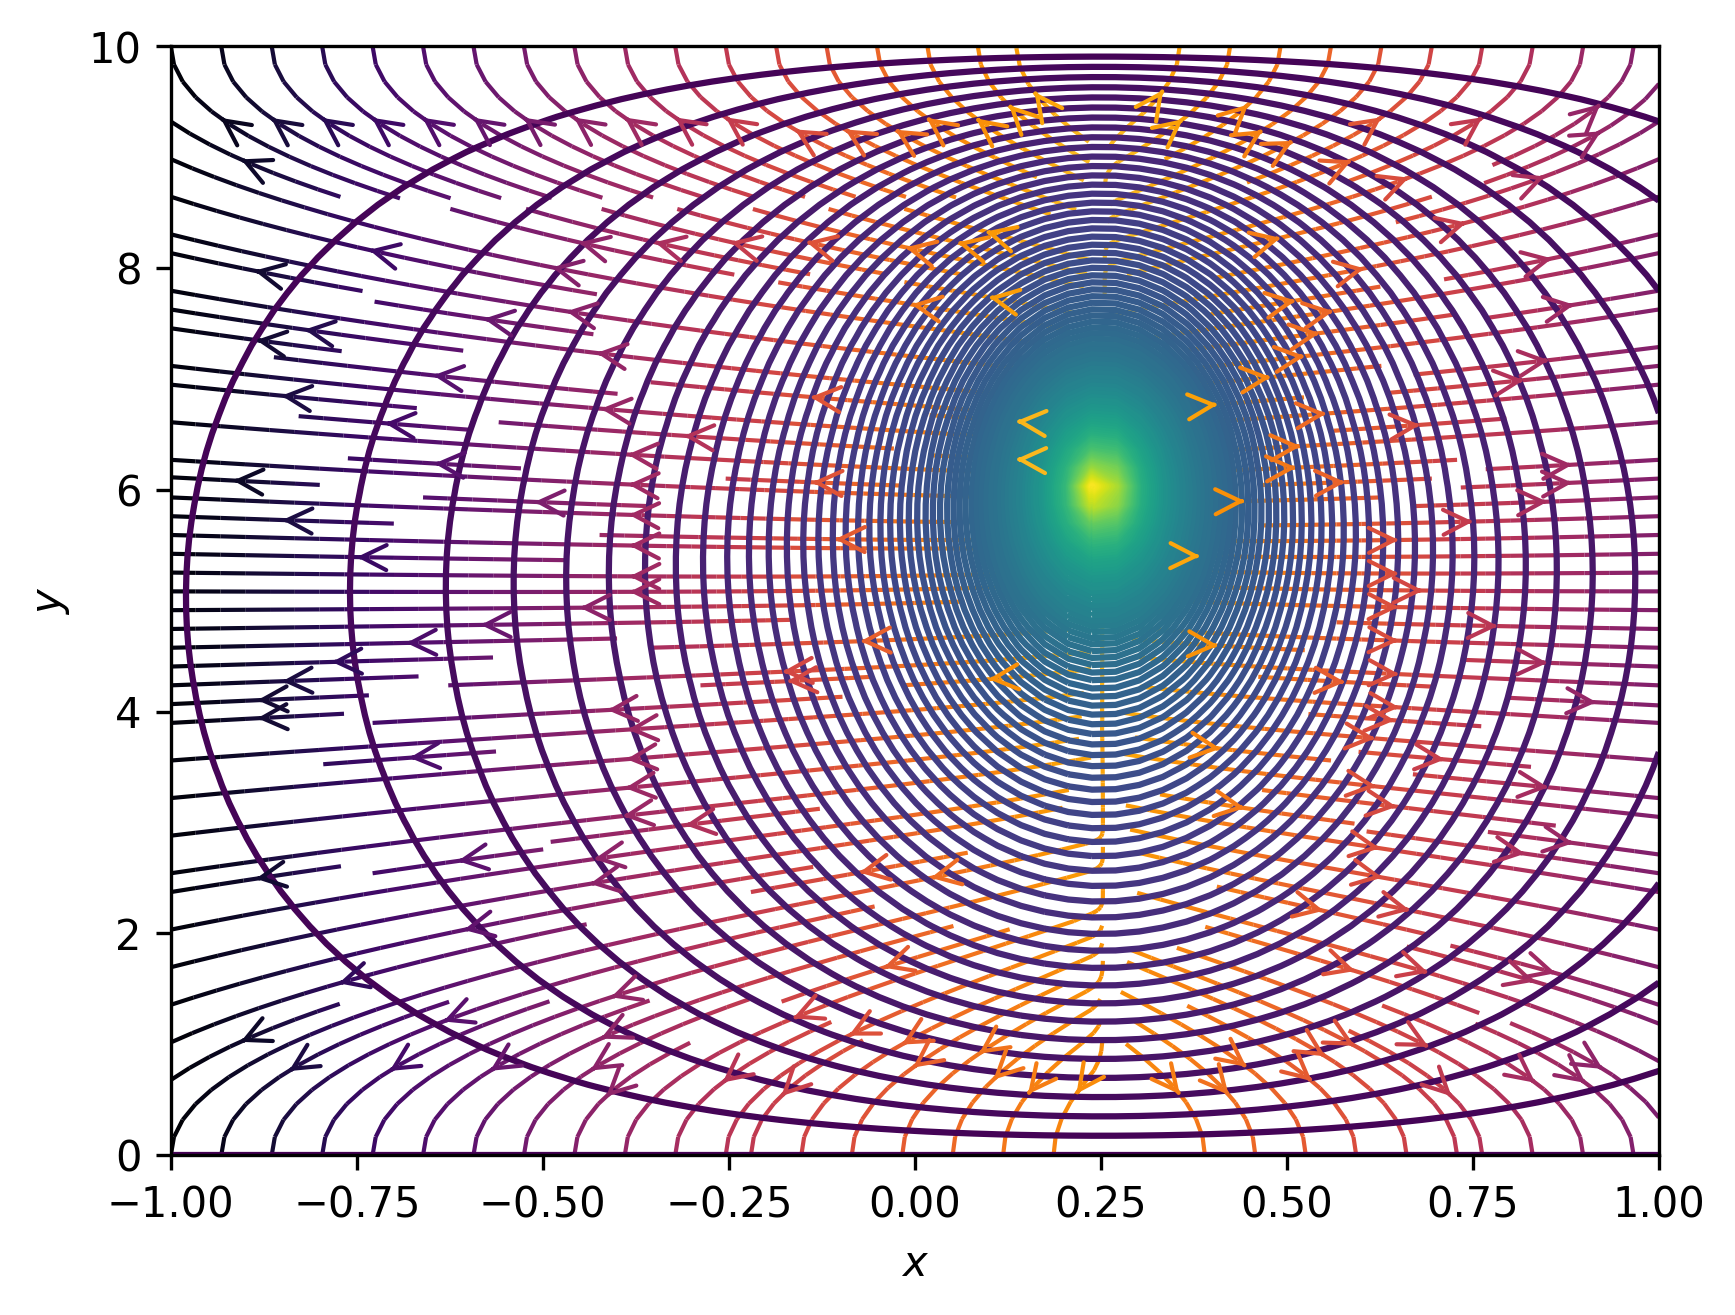
\includegraphics[width=\linewidth]{programs/estatic-wire-plates/plate-wire-200.png}}
    
\end{frame}
  
  \begin{frame}
    \frametitle{Geladene Kugelfläche}
\begin{itemize}[<+->]
\item Problem: Potential einer geladene Kugelfläche mit Radius $R$ und \alert{rotationssymmetrischer} Ladungsverteilung
  $$
  \laddichte{V} (\Ortsr[v]) =\laddichte{V} (r,\vartheta,\varphi) = \laddichte{F} (\textcolor{red}{\vartheta}) \delta(r-R) = \sigma(\vartheta) \delta(r-R) 
  $$
\item Idee: Unterteilung in \enquote{innen} und \enquote{außen}; $\sigma$ $\to$ Neumann Randbedingung bei $R$.
\item Potential ($\to$ Elektrostatik-VI: Orthogonale Funktionensysteme):
\begin{align*}
            \phi(r, \vartheta,\varphi) &= \sum_{l=0}^{\infty}\sum_{m=-l}^l  \underbrace{c_{lm} R_l(r)}_{R_{lm}(r)=c_{lm}(A r^l+ B r^{-(l+1)})} Y_{lm}(\vartheta,\varphi)\\
            &= \sum_{l=0}^{\infty}\sum_{m=-l}^l  (A_{lm} r^l+ B_{lm} r^{-(l+1)}) Y_{lm}(\vartheta,\varphi) \text{ mit } \\Y_{lm}(\vartheta,\varphi)&= \sqrt{\frac{2l+1}{4\pi}\frac{(l-m)!}{(l+m)!}} P_{lm}(\cos\vartheta) e^{jm\varphi}
\end{align*}
\end{itemize}
\end{frame}

\begin{frame}
 \begin{itemize}[<+->]
 \item Problem ist \alert{rotationssymmetrisch} bezüglich $\varphi$ $\to$ Lösung kann nicht von $\varphi$ abhängen $\to$ $m=0$:
   \begin{align*}
     \phi(r, \vartheta,\varphi) = \phi(r, \vartheta) &= \sum_{l=0}^{\infty} (A_{l} r^l+ B_{l} r^{-(l+1)}) Y_{l0}(\vartheta,\varphi)\\
                                                     &= \sum_{l=0}^{\infty} (A_{l} r^l+ B_{l} r^{-(l+1)}) \sqrt{\frac{2l+1}{4\pi}} \underbrace{P_{l0}(\cos\vartheta)}_{P_l (\cos\vartheta)}\\
     & = \sum_{l=0}^{\infty} (A_{l} r^l+ B_{l} r^{-(l+1)}) \frac{2l+1}{2} P_l (\cos\vartheta)
   \end{align*}
 \item Dabei sind $P_{l0}(x) = P_l(x)$ die \alert{Legendre-Polynome}:
   $$
   P_{l0}(x) = P_l(x) = \frac{1}{2^l l!} \frac{\upd^l}{\upd x^l} (x^2-1)^l \text{ voll. System auf } [-1,1]
   $$
 \item Orthogonalitätsrelation der Legendre Polynome:
   $$
   \int_{-1}^1 P_l(x)P_m(x) \upd x = \frac{2}{2l+1} \delta_{lm}
   $$
 \end{itemize}

\end{frame}

\begin{frame}
\begin{itemize}[<+->]
\item Da die Legendre-Polynome ein vollständiges System auf $[-1,1]$ (bezüglich $\cos\vartheta$ also $[0,\pi]$) sind, kann auch die Oberflächenladungsdichte nach diesen entwickelt werden:
  $$
  \sigma(\vartheta) = \sum_{l=0}^{\infty}  \frac{2l+1}{2} \sigma_l P_l (\cos\vartheta)
  $$
\item Multiplikation mit $P_m$, Integration und Nutzung der Orthogonalitätsrelation liefert:
  $$
  \sigma_l = \int_{-1}^{1} \sigma(\vartheta) P_l(\cos\vartheta) \upd \cos\vartheta
  $$
\item Offensichtlich sollte das Potential aufgeteilt werden in
  $$
  \phi(\Ortsr[v]) = \phi(r,\vartheta) = \begin{cases}
    \phi_- (r,\vartheta) = \sum_{l=0}^{\infty} (A_{l}^- r^l+ B_{l}^- r^{-(l+1)}) \frac{2l+1}{2} P_l (\cos\vartheta) & \text{ für } r < R \\
    \phi_+ (r,\vartheta)=\sum_{l=0}^{\infty} (A_{l}^+ r^l+ B_{l}^+ r^{-(l+1)}) \frac{2l+1}{2} P_l (\cos\vartheta) & \text{ für } r > R
    \end{cases}
    $$
  \item Keine Ladung im Ursprung $\to$ keine Singularität von $\phi_-(r\to 0) \Rightarrow \boxed{B_l^- =0}$
  \item Potential verschwindet im Unendlichen $\phi_+(r\to \infty) = 0  \Rightarrow \boxed{A_l^+ =0}$
    \item Stetigkeit bei $r=R$: $\left. A_{l}^- r^l\right|_{r=R} = \left. B_{l}^+ r^{-(l+1)}\right|_{r=R} \Rightarrow \boxed{B_{l}^+ = A_{l}^- R^{2l+1} } $  
 \end{itemize} 
\end{frame}

\begin{frame}
  \begin{itemize}[<+->]
  \item Nutzung der Neumann Randbedingung:
    \begin{align*}
      \sigma(\vartheta) &= -\varepsilon_0 \left.\left( \frac{\partial \phi_+}{\partial r} - \frac{\partial \phi_-}{\partial r}\right)\right|_{r=R} \\
                     & = \left. -\varepsilon_0 \sum_{l=0}^{\infty} \left( -(l+1) A_{l}^- R^{2l+1} r^{-(l+2)}- l A_{l}^- r^{l-1}\right) \frac{2l+1}{2} P_l (\cos\vartheta) \right|_{r=R} \\
      &= \varepsilon_0 \sum_{l=0}^{\infty} \frac{(2l+1)^2}{2} A_{l}^- R^{l-1} P_l (\cos\vartheta) 
    \end{align*}
  \item Andererseits gilt die Entwicklung: $\sigma(\vartheta) = \sum_{l=0}^{\infty}  \frac{2l+1}{2} \sigma_l P_l (\cos\vartheta)$, also:
    $$
    \varepsilon_0 (2l+1) A_{l}^- R^{l-1} = \sigma_l \Rightarrow \boxed{ A_{l}^- = \frac{1}{(2l+1)\varepsilon_0}\sigma_l  R^{-(l-1)}}
    $$
  \item Damit ist die Gesamtlösung gefunden:
    $$
    \phi(\Ortsr[v]) = \phi(r,\vartheta) =
    \begin{cases}
      \phi_-(r,\vartheta) & = \frac{R}{\varepsilon_0} \sum_{l=0}^{\infty} \frac{\sigma_l}{2} \left(\frac{r}{R}\right)^l P_l(\cos\vartheta) \text{ für } r<R\\ 
      \phi_+(r,\vartheta) & = \frac{R}{\varepsilon_0} \sum_{l=0}^{\infty} \frac{\sigma_l}{2} \left(\frac{R}{r}\right)^{l+1} P_l(\cos\vartheta) \text{ für } r>R\\ 
      \end{cases}
    $$
    \end{itemize}
  \end{frame}

 \begin{frame}
   \frametitle{Einfachster Fall: homogen geladene Kugel}
   \begin{itemize}[<+->]
   \item homogene Kugel: $\sigma(\vartheta) = \sigma = \frac{Q}{4\pi R^2}$
   \item Entwicklung von $\sigma(\vartheta)$: $\sigma(\vartheta) = \sum_{l=0}^\infty \frac{2l+1}{2}\sigma_l P_l(\cos(\vartheta))$:
     \begin{align*}
       \frac{Q}{4\pi R^2} & = \sum_{l=0}^\infty \frac{2l+1}{2}\sigma_l P_l(\cos(\vartheta)) \stackrel{l=0}{=} \frac{\sigma_0}{2}\\
       \sigma_0 &= \frac{2Q}{4\pi R^2}
     \end{align*}
   \item Damit Potentiale und Felder:
     \begin{align*}
       \phi_-(r) & = \frac{Q}{4\pi\varepsilon_0 R} & \phi_+(r) & = \frac{Q}{4\pi\varepsilon_0 r}\\
       \EFeld[v]_- (r) &= \vec{0} & \EFeld[v]_+ (r) &= \frac{Q}{4\pi\varepsilon_0} \frac{\Ortsr[v]}{r^3} 
       \end{align*}
     \end{itemize}
\end{frame}  

\input{finalframe.inc}
   
\end{document}